\chapter{Test Data Registers}
\label{chap:data-reg}

This chapter gives an overview of data registers and their operation. It contains the following sections:
\begin{itemize}
    \item \hyperref[sec:about-data-regs]{About Data Registers}
    \item \hyperref[sec:data-regs-types]{Types of Data Registers}
\end{itemize}

\newpage

\section{About Data Registers}
\label{sec:about-data-regs}

The test logic architecture contains two test data registers (TDRs); the bypass and boundary-scan registers. In addition, the designs of other standard optional test data registers are defined: the device identification, electronic chip identification, initialization data, initialization status, TMP status, and reset selection registers.

The bypass, boundary-scan, and optional test data registers are realized as a set of shift-register based elements connected in parallel between a common serial input and a common serial output. Selection of the register that forms the serial path at a given time is controlled from the instruction register.

\vspace{1.25cm}
\begin{figure}[H]
    \centering
    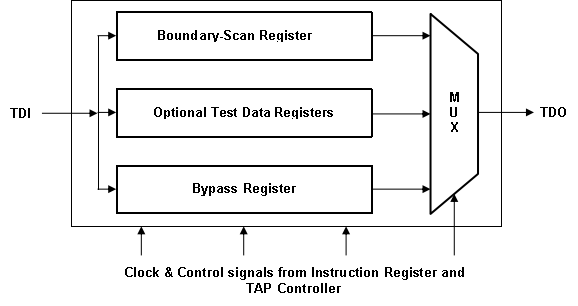
\includegraphics[width = 15cm]{images/test_data_registers.png}
    \vspace{1cm}
    \caption{JTAG Test data Registers Overview}
    \label{fig:data-regs-overview}
\end{figure}
\vspace{1cm}

Bypass Register provides a single-bit, which is the minimum length for any TDR serial connection through the circuit when none of the other test data registers is selected. This register can, for example, be used to allow test data to flow through a particular component to other components in a product without affecting the normal operation of the particular component.

Boundary-Scan Register allows testing of board interconnections, detecting typical production defects such as opens, shorts, and so on. It also allows access to the inputs and outputs of components when testing their system logic or sampling of signals flowing through the system inputs and outputs.

Boundary-scan register is not in the scope of current implementation. Only BYPASS, IDCODE, USERCODE, and USERDATA registers are implemented as a part of JTAG.

\section{Design of JTAG Register}

\vspace{1cm}
\begin{figure}[H]
    \centering
    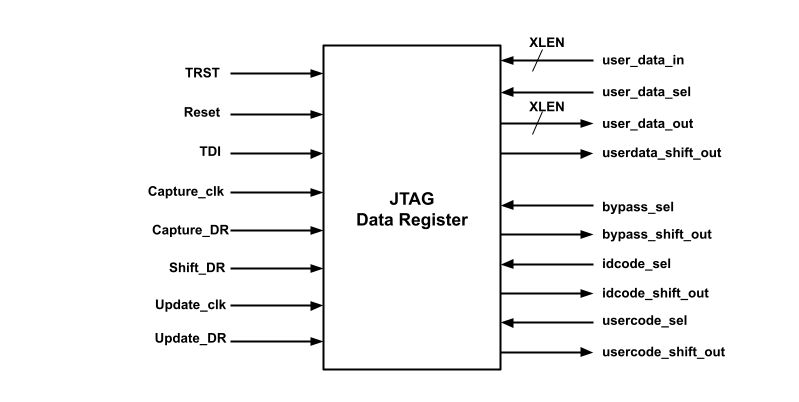
\includegraphics[width = 15cm]{images/jtag_data_register.png}
    \vspace{1cm}
    \caption{JTAG Test data Register}
    \label{fig:data-reg}
\end{figure}
\vspace{1cm}

\subsection{Data Register Ports}

\begin{longtable}{l l p{9.5cm}}
    \caption{Data Register port description}
    \label{tab:data-reg-ports}\\
    \hline
         \textbf{Port Name} & \textbf{Direction} & \textbf{Description}\\ \hline \hline
        \hyperref[subsec:trst]{TRST} & Input & Asynchronous Active low reset: If asserted default IDCODE Instruction is selected. \\ \hline
        Reset & Input & This signal is asserted when the state is in \texttt{TEST\_LOGIC\_RESET} State. \\ \hline
        \hyperref[subsec:tdi]{TDI} & Input & Test Data Input \\ \hline 
        Capture\_clk & Input & Capture\_clk (posedge of TCK) captures the data \\ \hline
        Capture\_DR & Input & Controls the Capture Operation of Data Register. Captures the data in the posedge of Capture\_clk if no TRST and Reset is there. \\ \hline
        Shift\_DR & Input & Controls the Shift Operation of Data Register. Shift the data bits from one register to another register in the posedge of Capture\_clk. \\ \hline
        Update\_clk & Input & Update\_clk (negedge of TCK) updates the data.\\ \hline
        Update\_DR & Input & Controls the Update Operation of Data Register. Update the data bits in the posedge of Update\_clk if no TRST. \\ \hline
        user\_data\_in & Input & XLEN bits of User Data Input coming from the top module specified by the user. \\ \hline
        user\_data\_sel & Input & Selects the USER DATA Register. \\ \hline
        user\_data\_out & Output & User Data Output Signal updates in the Update\_DR State. \\ \hline
        userdata\_shift\_out & Output & User Data Shift out bit shifted data bit in the Shift\_DR State.  \\ \hline
        bypass\_sel & Input & Selects the Bypass Register  \\ \hline
        bypass\_shift\_out & Output & Bypass shift bit in the Shift\_DR state.  \\ \hline
        idcode\_sel & Input & Selects the IDCODE Register. \\ \hline
        idcode\_shift\_out & Output & Idcode shift bit in the Shift\_DR State  \\ \hline
        usercode\_sel & Input & Selects the USER CODE Register.  \\ \hline
        usercode\_shift\_out & Output & User code shift bit in the Shift\_DR State.  \\ \hline
\end{longtable}

\section{Types of Data Registers}
\label{sec:data-regs-types}

The different types of Data Register are as follows:
\begin{enumerate}
    \item \hyperref[subsec:bypass-reg]{BYPASS register}
    \item \hyperref[subsec:idcode-reg]{IDCODE register}
    \item \hyperref[subsec:device-id-reg]{Device Identification register}
    \item \hyperref[subsec:userdata-reg]{USERDATA Register}
\end{enumerate}

\subsection{BYPASS register}
\label{subsec:bypass-reg}
The BYPASS mode is activated when an instruction code of all 1’s is loaded in the instruction register. In this register the scan data passes through a device once the TAP controller is in the SHIFT\_DR state. In this state, data signals are clocked into the bypass register from TDI on the rising edge of TCK and out of TDO on the falling edge of the same clock pulse.

\subsection{IDCODE register}
\label{subsec:idcode-reg}
The IDCODE instruction mode is used to identify the devices in an IEEE Std. 1149.1 chain. When IDCODE is selected, the device identification register is loaded with the 32-bit vendor-defined identification code (\texttt{32'h1495\_11c3}). The device ID register is connected between the TDI and TDO ports, and the device IDCODE is shifted out.

\subsection{Device Identification register}
\label{subsec:device-id-reg}
The USERCODE instruction mode is used to examine the user electronic signature (UES) within the devices along an IEEE Std. 1149.1 chain. When this instruction is selected, the device identification register is connected between the TDI and TDO ports. The user-defined UES is shifted into the device ID register in parallel from the 32-bit USERCODE register. The UES is then shifted out through the device ID register. The UES value is not user defined until after the device has been configured. Before configuration, the UES value is set to the default value.

\subsection{USERDATA Register}
\label{subsec:userdata-reg}
In this register 8 bit user data input value is captured in the Capture\_DR Stage and then shifted in the Shift\_DR Stage in the posedge of Capture\_clk if no TRST and Reset is there. The shifted bits are updated to user data output in the Update\_DR Stage in the posedge of Update\_clk.
